% ---------------------------------------------------
% ----- Introduction of the template
% ----- for Bachelor-, Master thesis and class papers
% ---------------------------------------------------
%  Created by C. Müller-Birn on 2012-08-17, CC-BY-SA 3.0.
%  Last upadte: C. Müller-Birn 2015-11-27 
%  Freie Universität Berlin, Institute of Computer Science, Human Centered Computing. 
%
\chapter{Introduction}
\label{chap:introduction}

\section{Project IKON}

This thesis has a direct application in a project which tries to explore potentials for knowledge transfer activities at a research museum. Project \textit{IKON} was started in cooperation with the German Natural History Museum in Berlin which houses more than 600 \tk{Right number?} scientists, PhD students and other staff. With that size of scientific staff the institution is a global player in research on evolution and biodiversity \cite{IntroducingMuseumFur}. Despite its importance in the research landscape, the museum is challenged with a lack of shared knowledge across working groups and organizational structures such as departments. In interviews researchers from the project were able to trace these problems back to the very intricate and complex layout of rooms and halls in the building which was originally constructed in 1810 \cite{140JahreAltes2018}. In order to mitigate this problem \autoref{pic:IKON-clusterview} shows one of the main deliverables of \textit{IKON} - a ML-driven data visualization which follows the path of knowledge at this research museum from its creation in projects over knowledge transfer activities, where multiple projects exchange their findings, to the final target group. Knowledge transfer is made explicitly visible by showing projects not in the predefined taxonomy of the museum, but instead in semantic relation to each other. This is accomplished by running all project abstracts through a topic modeling process consisting of four major components, as seen in \autoref{pic:general_topic_extraction_pipeline}. 

\section{Topic modeling}

A general topic modeling pipeline consists of four steps: 
\begin{enumerate}
	\item Document embedding
	\item Topic extraction
	\item Classification of documents
	\item Reduction into 2D
\end{enumerate}

Given an unlabeled corpus $C = \{D_1, ..., D_n\}$ consisting of $n$ documents $D_i = (t_1, ..., t_m)$, which in turn consists of a sequence of $m$ strings, also called tokens or words, the document embedding step assigns to each document a vector $v_D \in \mathbb{R}^e, e \in \mathbb{N}^+$. Semantically similar documents should also be closer in the embedded vector space with respect to a given distance measure than documents which are semantically not related. Therefore this step transforms a corpus into a matrix $(v_1, ..., v_n) \in \mathbb{R}^{e \times n}$.

Consuming the output from the previous step the topic extraction tries to uncover $k$ latent structures. We call these structures \textit{topics}. Mathematically speaking a topic is a probability distribution over a fixed set of input features. \cite{liuOverviewTopicModeling2016} These features can correspond to tokens, as it is the case in the later discussed Tfidf-BOW embedding, but this does not have to be the case. Therefore this step transforms the corpus from the embedding space of dimensionality $e \times n$, where each document is described as linear combination of features, to the latent space of dimensionality $k \times n$, where each document is described as a linear combination of latent topics. Since most often $k < e$ holds true, this can also be seen as a form of dimensionality reduction, which is again a form of feature extraction.

Using the document vectors in the latent space each document is assigned a label. This may happen in a supervised way if there are labels available for training purposes, but in most cases an unsupervised classification, also known as clustering, is used to group the documents.

Finally in order to visualize the high dimensional distribution of documents in the latent space another dimensionality reduction is used to project the documents to 2D.

\begin{figure}[t]
	\centering
	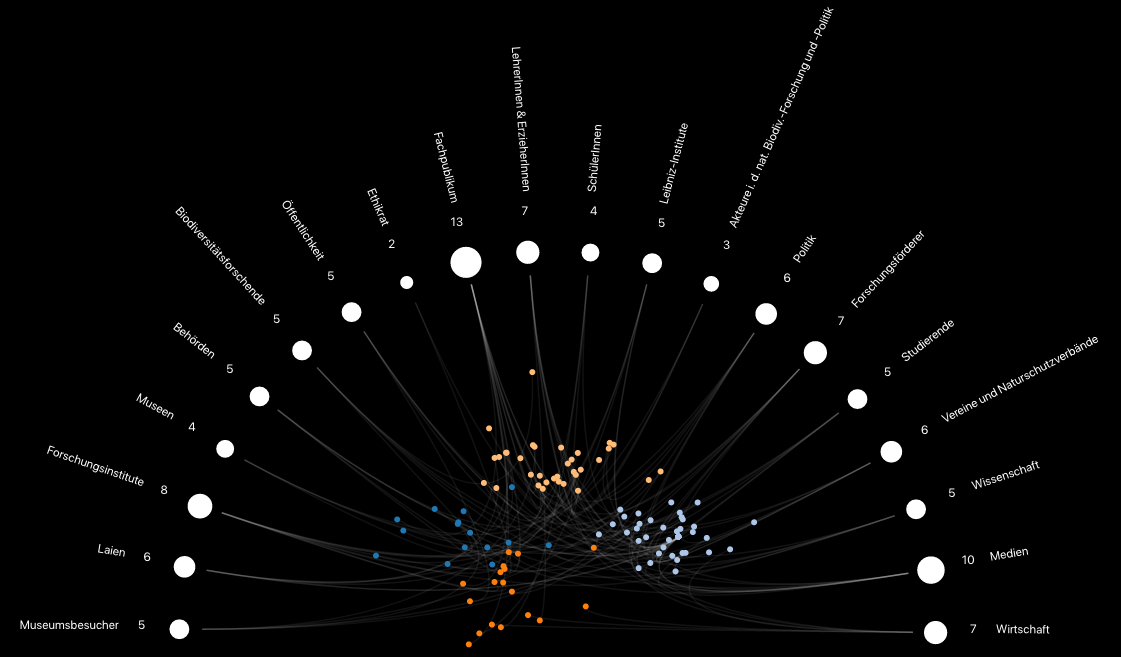
\includegraphics[width=400px]{../chapters/introduction/graphics/ikon-clusterview}
	\caption{\label{pic:IKON-clusterview} Screenshot of the cluster view of the IKON visualization}
\end{figure}

% Define block styles
\tikzstyle{decision} = [diamond, draw, fill=blue!20, 
text width=4.5em, text badly centered, node distance=3cm, inner sep=0pt]
\tikzstyle{block} = [rectangle, draw, fill=blue!20, 
text width=6em, text centered, rounded corners, minimum height=4em]
\tikzstyle{line} = [draw, -latex']
\tikzstyle{cloud} = [draw, ellipse,fill=red!20, node distance=3cm,
minimum height=2em]

\begin{figure}[t]
	\centering
	\begin{tikzpicture}[node distance = 4cm, auto]
	% Place nodes
	\node [block] (emb) {Document embedding};
	%\node [cloud, left of=emb] (expert) {expert};
	%\node [cloud, right of=emb] (system) {system};
	\node [block, right of=emb] (topic) {Topic extraction};
	\node [block, right of=topic, above of=topic] (cluster) {Classification of documents};
	\node [block, right of=topic, below of=topic] (2D) {Reduction into 2D};
	% Draw edges
	\path [line] (emb) -- (topic);
	\path [line] (topic) -- (cluster);
	\path [line] (topic) -- (2D);
	%\path [line] (identify) -- (evaluate);
	%\path [line] (update) |- (identify);
	%\path [line,dashed] (system) |- (evaluate);
	\end{tikzpicture}
	\caption{\label{pic:general_topic_extraction_pipeline} Components of a general topic extraction pipeline}
\end{figure}

Based in first interviews and conceptual work the researchers from project IKON hypothesize that the scientists from the museum, as non-technical experts, will have a hard time interpreting and understanding the output generated by the pipeline. Furthermore each component in \autoref{pic:general_topic_extraction_pipeline} introduces additional parameters which influence the results generated by the pipeline. 

In order to lay the groundwork for this thesis and understand the challenges which scientists face while interacting with the visualization I carried out a workshop with the researchers from project \textit{IKON}. In the beginning I asked them which kind of hardships they, based on their past experiences and interviews, hypothesize during the interaction between user and visualization. Followed by an explanation of \autoref{pic:general_topic_extraction_pipeline} we discussed how these challenges may correlate with goals and questions. Following a description of the key questions each question was categorized according to the pipeline step, , as seen in \autoref{tab:overview_viz_questions}, which may contribute information in order to support the user in answering his question.

\begin{table}
	\centering
	\begin{tabular}{ c | c }
		\hline 
		Question & Applicable pipeline component \\ \hline
		How does the research landscape look like \\ and on what kind of topics are prominent? & Topic Extraction \\ \hline
		What does a cluster mean? & Classification \\ \hline
		What does the distance between \\ clusters/projects mean? & Topic Extraction / Reduction into 2D \\ \hline
		How similar are two projects/clusters? & Topic Extraction \\
		\hline
	\end{tabular}
	\caption{\label{tab:overview_viz_questions} Table showing the sourced questions and the pipeline step which could provide an answer}
\end{table} 

\section{Interpretability}

With the surge of the application of machine learning (ML) systems in our daily life there is an increasing demand to make operation and results of these systems interpretable for people with different backgrounds (ML experts, non-technical experts etc.). Contrary to these efforts, interpretability as term has become an ill-defined objective \cite{liptonMythosModelInterpretability2016a} for research and development in ML algorithms since there is no widely agreed upon definition of it. This leads to a very fragmented nature of the field. 

Miller et al. \cite{millerExplainableAIBeware2017} support this point by conducting a literature study and uncovering that interpretability research is rarely influenced by insights from the humanities, especially connected fields as explainability or causality research.

%\tk{Interpretation of machine learning (ML) results is a major challenge for humans, especially for non-technical experts [ref]. Research on interpretability\footnote{Which we position to be a high-level precondition for Explainability from the XAI \cite{gunning_broad_2016} and Fairness, Accountability and Transparency, from the FAT-ML discourse \cite{kohli_translation_2018}.} in the ML community has focused on developing interpretability techniques, i.e. specific technical approaches to generate explanations\footnote{Which we define as instances of interpretability techniques.} for ML results. However, applications of these techniques are predominantly concerned with making particular model features understandable, rather than supporting the interpretation of ML-driven systems in a specific context of use. At the same time, research in the HCI domain often remains on a formal, algorithmic level---explanations tend to be technical and tailored to an expert audience, mirroring the technical focus of ML research. Realistic use cases and qualitative, context-aware evaluations to inform the selection and design of interpretability techniques remain rare.  While we do not see complete transparency as a prerequisite for interpretability we hypothesize that in general, since interpretation is dependent on context, interpretability techniques cannot be fully context agnostic either. Therefore, our general approach is to research interpretability from a context-aware perspective, i.e. we explore how interpretability can be operationalized in a specified, well-defined domain context.}

